%!TEX root = ../main.tex
\chapter{Physical Laws of Photon Simulation}
\label{chapter9}

This chapter introduces the physical and mathematical principles underlying the
simulation of X-ray imaging. Central to this is the modeling of individual
photon interactions with matter, including attenuation and scattering processes.
These interactions are inherently stochastic due to the quantum nature of
radiation-matter interactions. The stochastic nature of photons and their interactions with matter is modeled using monte Carlo methods of uniformly distributed values between 0 and 1, which are then transformed to follow the physical probability distributions relevant to the specific interactions being simulated. This approach allows for a realistic representation of photon transport and interaction within the imaging system.

\begin{figure}[H]
    \centering
    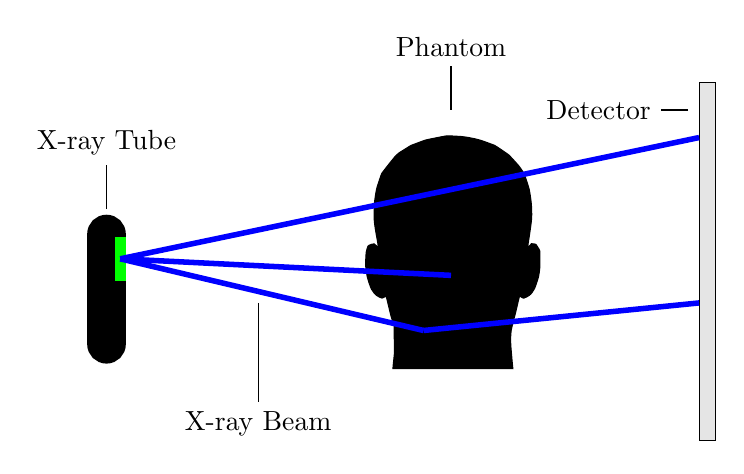
\begin{tikzpicture}[scale=.07]
        \draw[fill=black, rounded corners=5pt, line width=4] (-50,-40) rectangle (-45,-15);
        \draw[draw=green, line width=4] (-45,-18) -- (-45,-26);

        
        \draw[fill=gray!20] (60,10) rectangle (63,-55);
        
        \draw[fill=black]
        (349.5pt, -1.599976pt) .. controls (310.3pt, -9.299927pt) and (295pt,
        -12.79993pt) .. (287.5pt, -15.59998pt) -- (287.5pt, -15.59998pt) --
        (287.5pt, -15.59998pt) -- (287.5pt, -15.59998pt) .. controls (261.5pt,
        -25.09998pt) and (221.4pt, -40.19995pt) .. (219.6pt, -41.19995pt) --
        (219.6pt, -41.19995pt) -- (219.6pt, -41.19995pt) -- (219.6pt,
        -41.19995pt) .. controls (216.9pt, -42.59998pt) and (168.1pt, -73pt) ..
        (156.8pt, -80.29993pt) -- (156.8pt, -80.29993pt) -- (156.8pt,
        -80.29993pt) -- (156.8pt, -80.29993pt) .. controls (149.5pt, -85pt) and
        (146.4pt, -88pt) .. (138pt, -98.09998pt) -- (138pt, -98.09998pt) --
        (138pt, -98.09998pt) -- (138pt, -98.09998pt) .. controls (116.2pt,
        -124.2999pt) and (79.00001pt, -171.4999pt) .. (69.3pt, -185.4999pt) --
        (69.3pt, -185.4999pt) -- (69.3pt, -185.4999pt) -- (69.3pt, -185.4999pt)
        .. controls (67.3pt, -188.2999pt) and (50.10001pt, -239.1pt) .. (44.5pt,
        -258.4999pt) -- (44.5pt, -258.4999pt) -- (44.5pt, -258.4999pt) --
        (44.5pt, -258.4999pt) .. controls (40.3pt, -273.2pt) and (32.9pt,
        -320.7pt) .. (30.9pt, -345.9999pt) -- (30.9pt, -345.9999pt) -- (30.9pt,
        -345.9999pt) -- (30.9pt, -345.9999pt) .. controls (30.3pt, -353.9999pt)
        and (29.7pt, -374.2pt) .. (29.7pt, -390.9999pt) -- (29.7pt, -390.9999pt)
        -- (29.7pt, -390.9999pt) -- (29.7pt, -390.9999pt) .. controls (29.6pt,
        -418.2pt) and (29.9pt, -423.9pt) .. (32.2pt, -443.6pt) -- (32.2pt,
        -443.6pt) -- (32.2pt, -443.6pt) -- (32.2pt, -443.6pt) .. controls
        (33.7pt, -455.7pt) and (37.8pt, -482.1pt) .. (41.4pt, -502.1pt) --
        (41.4pt, -502.1pt) -- (41.4pt, -502.1pt) -- (41.4pt, -502.1pt) ..
        controls (49.10001pt, -544.8pt) and (51pt, -556.7pt) .. (51pt, -563.4pt)
        -- (51pt, -563.4pt) -- (51pt, -563.4pt) -- (51pt, -563.4pt) -- (51pt,
        -568.4pt) -- (51pt, -568.4pt) -- (40.6pt, -558.1pt) -- (40.6pt,
        -558.1pt) -- (40.6pt, -558.1pt) -- (40.6pt, -558.1pt) .. controls (29pt,
        -546.7pt) and (31.3pt, -547.4pt) .. (17.2pt, -551.1pt) -- (17.2pt,
        -551.1pt) -- (17.2pt, -551.1pt) -- (17.2pt, -551.1pt) .. controls
        (8.200001pt, -553.4999pt) and (0.500001pt, -557.3pt) .. (-1.499999pt,
        -560.3pt) -- (-1.499999pt, -560.3pt) -- (-1.499999pt, -560.3pt) --
        (-1.499999pt, -560.3pt) .. controls (-3.4pt, -563.2pt) and (-8.7pt,
        -580.7pt) .. (-10.5pt, -590.3pt) -- (-10.5pt, -590.3pt) -- (-10.5pt,
        -590.3pt) -- (-10.5pt, -590.3pt) .. controls (-11.3pt, -594.3pt) and
        (-12.5pt, -610.9pt) .. (-13.2pt, -627.3pt) -- (-13.2pt, -627.3pt) --
        (-13.2pt, -627.3pt) -- (-13.2pt, -627.3pt) -- (-14.4pt, -657.1pt) --
        (-14.4pt, -657.1pt) -- (-11.1pt, -683.8pt) -- (-11.1pt, -683.8pt) --
        (-11.1pt, -683.8pt) -- (-11.1pt, -683.8pt) .. controls (-7.4pt,
        -712.8pt) and (-5.099999pt, -723.2pt) .. (4.400002pt, -751.5pt) --
        (4.400002pt, -751.5pt) -- (4.400002pt, -751.5pt) -- (4.400002pt,
        -751.5pt) .. controls (14.6pt, -781.8pt) and (17.2pt, -786.9pt) ..
        (30.8pt, -803.4pt) -- (30.8pt, -803.4pt) -- (30.8pt, -803.4pt) --
        (30.8pt, -803.4pt) .. controls (38.2pt, -812.5pt) and (43.2pt, -816.3pt)
        .. (56.5pt, -823pt) -- (56.5pt, -823pt) -- (56.5pt, -823pt) -- (56.5pt,
        -823pt) .. controls (71.00001pt, -830.3pt) and (71.7pt, -830.3pt) ..
        (82.4pt, -823.5pt) -- (82.4pt, -823.5pt) -- (82.4pt, -823.5pt) --
        (82.4pt, -823.5pt) .. controls (89.2pt, -819.1pt) and (91.40001pt,
        -818.1pt) .. (92.10001pt, -819.2pt) -- (92.10001pt, -819.2pt) --
        (92.10001pt, -819.2pt) -- (92.10001pt, -819.2pt) .. controls
        (92.90001pt, -820.4pt) and (94.60001pt, -827.3pt) .. (107.5pt, -882pt)
        -- (107.5pt, -882pt) -- (107.5pt, -882pt) -- (107.5pt, -882pt) ..
        controls (115.6pt, -916.2pt) and (119.4pt, -930.2pt) .. (126.5pt,
        -952pt) -- (126.5pt, -952pt) -- (126.5pt, -952pt) -- (126.5pt, -952pt)
        -- (132.8pt, -971.5pt) -- (132.8pt, -971.5pt) -- (134pt, -1040.5pt) --
        (134pt, -1040.5pt) -- (135.1pt, -1109.5pt) -- (135.1pt, -1109.5pt) --
        (131.1pt, -1149.1pt) -- (131.1pt, -1149.1pt) -- (131.1pt, -1149.1pt) --
        (131.1pt, -1149.1pt) .. controls (128.8pt, -1170.9pt) and (127pt,
        -1189.7pt) .. (127pt, -1190.9pt) -- (127pt, -1190.9pt) -- (127pt,
        -1190.9pt) -- (127pt, -1190.9pt) -- (127pt, -1193pt) -- (127pt, -1193pt)
        -- (436.5pt, -1193pt) -- (436.5pt, -1193pt) -- (746.0001pt, -1193pt) --
        (746.0001pt, -1193pt) -- (745.5001pt, -1189.3pt) -- (745.5001pt,
        -1189.3pt) -- (745.5001pt, -1189.3pt) -- (745.5001pt, -1189.3pt) ..
        controls (744.0001pt, -1177.4pt) and (737.3pt, -1102pt) .. (735.4pt,
        -1075.5pt) -- (735.4pt, -1075.5pt) -- (735.4pt, -1075.5pt) -- (735.4pt,
        -1075.5pt) .. controls (733.4pt, -1047.1pt) and (733.9pt, -1024.6pt) ..
        (737.0001pt, -996pt) -- (737.0001pt, -996pt) -- (737.0001pt, -996pt) --
        (737.0001pt, -996pt) .. controls (739.5001pt, -972.6pt) and (740.1pt,
        -969.7pt) .. (748.0001pt, -946pt) -- (748.0001pt, -946pt) --
        (748.0001pt, -946pt) -- (748.0001pt, -946pt) .. controls (754.0001pt,
        -928.2pt) and (758.0001pt, -912.4pt) .. (771.1pt, -855.5pt) -- (771.1pt,
        -855.5pt) -- (771.1pt, -855.5pt) -- (771.1pt, -855.5pt) .. controls
        (778.4pt, -823.6pt) and (779.7pt, -819pt) .. (781.3pt, -819pt) --
        (781.3pt, -819pt) -- (781.3pt, -819pt) -- (781.3pt, -819pt) .. controls
        (782.0001pt, -819pt) and (785.3pt, -820.6pt) .. (788.6pt, -822.6pt) --
        (788.6pt, -822.6pt) -- (788.6pt, -822.6pt) -- (788.6pt, -822.6pt) ..
        controls (799.4pt, -829.3pt) and (799.7pt, -829.4pt) .. (804.4pt,
        -828pt) -- (804.4pt, -828pt) -- (804.4pt, -828pt) -- (804.4pt, -828pt)
        .. controls (810.3pt, -826.3pt) and (825.2001pt, -818.4pt) .. (831.8pt,
        -813.5pt) -- (831.8pt, -813.5pt) -- (831.8pt, -813.5pt) -- (831.8pt,
        -813.5pt) .. controls (839.3pt, -808.1pt) and (852.1pt, -791.1pt) ..
        (857.6pt, -779.5pt) -- (857.6pt, -779.5pt) -- (857.6pt, -779.5pt) --
        (857.6pt, -779.5pt) .. controls (862.1pt, -769.9pt) and (873.3pt,
        -736.7pt) .. (877.4pt, -721pt) -- (877.4pt, -721pt) -- (877.4pt, -721pt)
        -- (877.4pt, -721pt) .. controls (878.7001pt, -715.8pt) and (881.0001pt,
        -703.8pt) .. (882.4pt, -694.3pt) -- (882.4pt, -694.3pt) -- (882.4pt,
        -694.3pt) -- (882.4pt, -694.3pt) .. controls (884.9pt, -677.7pt) and
        (885.0001pt, -675.5pt) .. (885.0001pt, -632pt) -- (885.0001pt, -632pt)
        -- (885.0001pt, -632pt) -- (885.0001pt, -632pt) -- (885.0001pt,
        -586.8pt) -- (885.0001pt, -586.8pt) -- (881.0001pt, -576.7pt) --
        (881.0001pt, -576.7pt) -- (881.0001pt, -576.7pt) -- (881.0001pt,
        -576.7pt) .. controls (877.2001pt, -567.1pt) and (875.4pt, -564.2pt) ..
        (867.1pt, -554.2pt) -- (867.1pt, -554.2pt) -- (867.1pt, -554.2pt) --
        (867.1pt, -554.2pt) .. controls (863.5001pt, -549.8pt) and (862.9pt,
        -549.6pt) .. (848.9pt, -548.6pt) -- (848.9pt, -548.6pt) -- (848.9pt,
        -548.6pt) -- (848.9pt, -548.6pt) -- (842.3pt, -548.1pt) -- (842.3pt,
        -548.1pt) -- (834.4pt, -556.1pt) -- (834.4pt, -556.1pt) -- (834.4pt,
        -556.1pt) -- (834.4pt, -556.1pt) .. controls (830.1pt, -560.4999pt) and
        (825.3pt, -564.9999pt) .. (823.8pt, -566.1pt) -- (823.8pt, -566.1pt) --
        (823.8pt, -566.1pt) -- (823.8pt, -566.1pt) .. controls (821.4pt,
        -567.8pt) and (821.2001pt, -567.9pt) .. (821.6pt, -566.3pt) -- (821.6pt,
        -566.3pt) -- (821.6pt, -566.3pt) -- (821.6pt, -566.3pt) .. controls
        (823.1pt, -559.7pt) and (836.5001pt, -470.9pt) .. (839.0001pt,
        -450.9999pt) -- (839.0001pt, -450.9999pt) -- (839.0001pt, -450.9999pt)
        -- (839.0001pt, -450.9999pt) .. controls (843.3pt, -415.4pt) and
        (843.8pt, -406.4999pt) .. (842.9pt, -377.9999pt) -- (842.9pt,
        -377.9999pt) -- (842.9pt, -377.9999pt) -- (842.9pt, -377.9999pt) ..
        controls (841.8pt, -344.7pt) and (840.7001pt, -332.9pt) .. (835.9pt,
        -301.1pt) -- (835.9pt, -301.1pt) -- (835.9pt, -301.1pt) -- (835.9pt,
        -301.1pt) .. controls (830.4pt, -264.7999pt) and (831.3pt, -268.4pt) ..
        (815.5001pt, -219.9pt) -- (815.5001pt, -219.9pt) -- (815.5001pt,
        -219.9pt) -- (815.5001pt, -219.9pt) -- (805.2001pt, -188.4pt) --
        (805.2001pt, -188.4pt) -- (794.7pt, -171.9pt) -- (794.7pt, -171.9pt) --
        (794.7pt, -171.9pt) -- (794.7pt, -171.9pt) .. controls (788.8pt,
        -162.8999pt) and (780.5001pt, -151.2pt) .. (776.2pt, -146pt) --
        (776.2pt, -146pt) -- (776.2pt, -146pt) -- (776.2pt, -146pt) .. controls
        (769.8pt, -138.2pt) and (745.9pt, -112pt) .. (726.5001pt, -91.29993pt)
        -- (726.5001pt, -91.29993pt) -- (726.5001pt, -91.29993pt) --
        (726.5001pt, -91.29993pt) .. controls (724.3pt, -89pt) and (706.8pt,
        -76.69995pt) .. (687.5001pt, -63.8999pt) -- (687.5001pt, -63.8999pt) --
        (687.5001pt, -63.8999pt) -- (687.5001pt, -63.8999pt) -- (652.6pt,
        -40.69995pt) -- (652.6pt, -40.69995pt) -- (626.0001pt, -30.79993pt) --
        (626.0001pt, -30.79993pt) -- (626.0001pt, -30.79993pt) -- (626.0001pt,
        -30.79993pt) .. controls (585.2pt, -15.49988pt) and (570pt, -10.69995pt)
        .. (545pt, -5.499878pt) -- (545pt, -5.499878pt) -- (545pt, -5.499878pt)
        -- (545pt, -5.499878pt) .. controls (512.4pt, 1.200073pt) and (497pt,
        3.800049pt) .. (481.9pt, 5.000122pt) -- (481.9pt, 5.000122pt) --
        (481.9pt, 5.000122pt) -- (481.9pt, 5.000122pt) .. controls (460.8pt,
        6.600098pt) and (415.2pt, 9.000122pt) .. (408pt, 8.900024pt) -- (408pt,
        8.900024pt) -- (408pt, 8.900024pt) -- (408pt, 8.900024pt) .. controls
        (404.2pt, 8.800049pt) and (380pt, 4.500122pt) .. (349.5pt, -1.599976pt)
        -- cycle ;
        \draw[blue, line width=2] (-45,-22) -- (60,0);
        \draw[blue, line width=2] (-45,-22) -- (10,-35);
        \draw[blue, line width=2] (-45,-22) -- (15,-25);
        \draw[blue, line width=2] (10,-35) -- (60,-30);

        \draw (-47.5,-13) -- (-47.5,-5) node[above] {X-ray Tube};
        \draw (15,5) -- (15,13) node[above] {Phantom};
        \draw (58,5) -- (53,5) node [left] {Detector};
        \draw (-20,-30) -- (-20,-48) node[below] {X-ray Beam};
    \end{tikzpicture}
    \caption{Schematic illustration of photon transport in X-ray imaging.}
    \label{fig:photon_transport}
\end{figure}

In a typical simulation workflow, individual photons are emitted from the X-ray
tube and propagate through air before reaching the phantom. Upon entering the
phantom, they may interact with the material through scattering or absorption,
depending on the local composition of the tissue and photon energy. Only a
fraction of the photons will exit the phantom, continue their path through air,
and ultimately reach the detector, contributing to the final image formation.

The simulation framework described here forms the basis for all subsequent
analyses presented in this thesis.


%-------------------------------------------------------------------------------%	SECTION 2
\section{X-Ray Tube Spectrum}
\label{sec:xray_tube_spectrum}
%-------------------------------------------------------------------------------

X-ray beams are generated within evacuated glass tubes containing several
critical components that convert electrical energy into X-ray photons and heat.
The X-ray tube acts as an energy converter, where the vast majority of the input
energy is transformed into heat and only a small fraction becomes useful
radiation. The following Figure~\ref{fig:xray_tube} illustrates the basic
construction of an X-ray tube as in \cite{poludniowski2022calculating}

\begin{figure}[H]
    \centering
    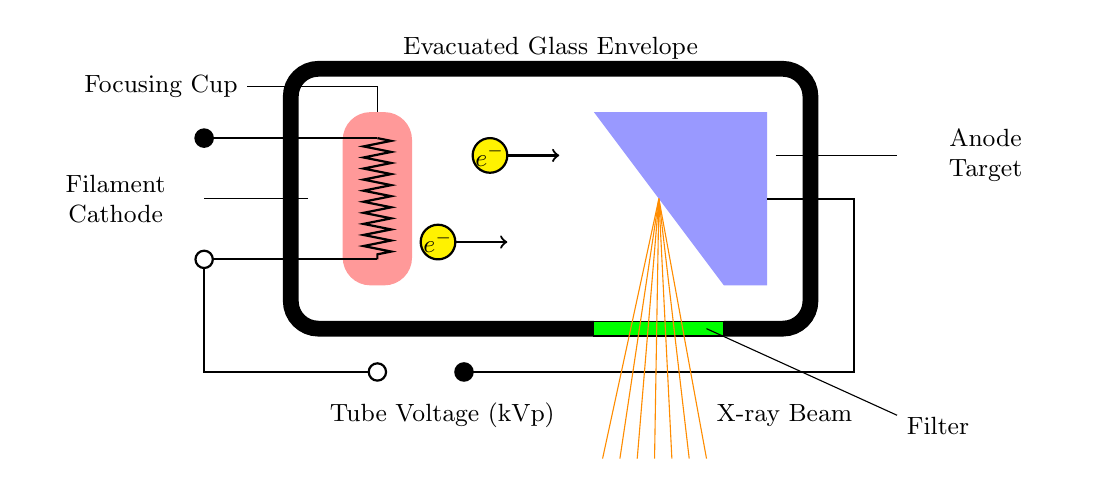
\begin{tikzpicture}[scale=1.1, every node/.style={font=\small}]
        % Glass envelope
        \draw[line width=2mm, rounded corners=10pt] (.5,-1.5) -- (-3,-1.5) -- (-3,1.5) -- (3,1.5) -- (3,-1.5) -- (2,-1.5);
        % Optional: dashed or lighter line to indicate the open section
        \draw[fill=green] (0.5,-1.415) rectangle (2,-1.585);
        \node[above] at (0,1.5) {Evacuated Glass Envelope};
        
        % Focusing Cup
        \draw[rounded corners=10pt, fill=red!40, draw=none] (-2.4,1) rectangle (-1.6,-1);
        \draw (-2,1) -- (-2,1.3) -- (-3.5,1.3) node [left] {Focusing Cup};

        % Filament (cathode)
        \draw[thick] (-4,.7) -- (-2,.7);
        \draw[thick, fill=black] (-4,.7) circle [radius=0.1];
        \draw[thick] (-4,-.7) -- (-2,-.7);
        \draw[thick] (-2,-2) -- (-4,-2) -- (-4,-.7);
        \draw[thick, fill=white] (-4,-.7) circle [radius=0.1];
        \draw[thick, decorate, decoration={zigzag, segment length=4pt, 
        amplitude=5pt}] (-2,.7) -- (-2,-.7);
        \draw (-2.8,0) -- (-4,0) node[left, align=center, text width=2cm] {Filament\\Cathode};

        % Anode Target
        \draw[fill=blue!40, draw=none] (.5,1) -- (2.5,1) -- (2.5,-1) -- (2,-1) -- cycle;
        \draw (2.6,.5) -- (4,.5) node[right, align=center, text width=2cm] {Anode\\Target};

        % Anode Voltage
        \draw[thick] (2.5,0) -- (3.5,0) -- (3.5,-2) -- (-1,-2);
        \draw[thick, fill=black] (-1,-2) circle [radius=0.1];
        \draw[thick, fill=white] (-2,-2) circle [radius=0.1];
        \node[below, align=center, text height=.5cm] at (-1.25,-2) {Tube Voltage (kVp)};

        % Electrons
        \draw[thick,->] (-1.3,-.5) -- (-.5,-.5);
        \draw[thick, fill=yellow] (-1.3,-.5) circle [radius=0.2] node[font=\small] {$e^{\text{-}}$};
        \draw[thick,->] (-.7,.5) -- (.1,.5);
        \draw[thick, fill=yellow] (-.7,.5) circle [radius=0.2] node[font=\small] {$e^{\text{-}}$};

        % Photon Beam
        \draw[orange!90!yellow] (.6,-3) -- (1.25,0);
        \draw[orange!90!yellow] (.8,-3) -- (1.25,0);
        \draw[orange!90!yellow] (1,-3) -- (1.25,0);
        \draw[orange!90!yellow] (1.2,-3) -- (1.25,0);
        \draw[orange!90!yellow] (1.4,-3) -- (1.25,0);
        \draw[orange!90!yellow] (1.6,-3) -- (1.25,0);
        \draw[orange!90!yellow] (1.8,-3) -- (1.25,0);
        \node[right, below, align=center, text height=.5cm] at (2.7,-2) {X-ray Beam};
        \draw (1.8,-1.5) -- (4,-2.5) node[right, align=center, text height=.5cm] {Filter};
    \end{tikzpicture}
    \caption{Schematic of an X-ray tube with filter.}
    \label{fig:xray_tube}
\end{figure}

To capture this randomness, Monte Carlo methods
are employed. In such simulations, random numbers—typically sampled uniformly
from the interval $[0,1]$ are transformed into physically meaningful
quantities according to the relevant probability distributions. This
probabilistic modeling enables realistic simulation of photon transport and
forms the basis for the analyses presented in this thesis.

The key components are:

\begin{itemize}
    \item \textbf{Filament (Cathode):} A tungsten wire filament serves as the
    electron source through thermionic emission. When a current of approximately
    3--6\,A passes through it, the filament reaches incandescence, releasing
    electrons from its surface. These free electrons form a cloud near the
    cathode until they are accelerated toward the anode by the applied high
    voltage.

    \item \textbf{Focusing Cup:} The filament is embedded in a negatively
    charged, nickel-made focusing cup. Its function is to electrostatically
    shape and direct the electron stream toward the anode's focal spot, thereby
    influencing the resolution and size of the resulting X-ray beam.

    \item \textbf{Anode Target:} The anode consists of a tungsten target, often
    embedded in a copper support. Tungsten is used for its high atomic number
    and melting point, enhancing X-ray production and durability. The copper
    base improves heat dissipation. Typically, less than 1\% of the electron
    energy is converted into X-rays, with the remainder generating heat that
    must be effectively managed.

    \item \textbf{Evacuated Glass Envelope:} All components are sealed within a
    borosilicate glass or metal-ceramic housing evacuated to a low pressure
    (typically $10^{-5}$ to $10^{-7}$\,hPa). The vacuum allows unimpeded
    electron flow and prevents arcing. The housing is usually immersed in
    insulating oil to provide thermal and electrical isolation.

    \item \textbf{Filter (Filtration):} A filter is positioned at the tube exit,
    between the anode target and the patient, to selectively absorb low-energy
    photons. These photons contribute little to image formation but
    significantly increase patient dose. Their removal (beam hardening) improves
    image quality by reducing scatter and enhancing contrast. Common filter
    materials are aluminum, copper and molybdenum; in this thesis, a clinical
    setup with $1$\,mm aluminum (Al) and $0.2$\,mm copper (Cu) is used
    \cite{poludniowski2022calculating,steidel2022dose}.
\end{itemize}

When high-energy electrons strike the tungsten target, X-ray photons are
produced through two primary mechanisms:

\begin{itemize}
    \item \textbf{Bremsstrahlung (Braking Radiation):} This accounts for
    approximately 80\% of X-ray production. When electrons pass close to
    tungsten nuclei, they are decelerated by the electrostatic attraction,
    causing them to lose kinetic energy that is emitted as X-ray photons. This
    process produces a continuous spectrum of X-ray energies from near zero up
    to the maximum electron energy.

    \item \textbf{Characteristic Radiation:} When high-energy electrons eject
    inner-shell electrons from tungsten atoms, vacancies are created in the K or
    L shells. These vacancies are subsequently filled by electrons from outer
    shells and the resulting energy difference is emitted as an X-ray photon
    with a discrete, element-specific energy. The corresponding peaks in the
    spectrum therefore occur at the differences of the binding energies of the
    involved shells. For reference, the atomic model of tungsten is shown in
    Figure~\ref{fig:tungsten_atomic_model_bohr} and the approximate binding energies
    of its shells and subshells are listed in
    Table~\ref{tab:tungsten_binding_energies}.

    From these binding energies, the main characteristic line energies can be
    derived. For example, the K$\alpha_1$ line corresponds to an electron
    transition from the L$_3$ subshell into the K-shell (69.5$-$10.2\,keV
    $\approx$ 59.3\,keV), the K$\alpha_2$ line results from the L$_2
    \rightarrow$ K transition (69.5$-$11.5\,keV $\approx$ 58.0\,keV) and the
    K$\beta_1$ line originates from the M$_2/M_3 \rightarrow$ K transition
    (69.5$-$2.3\,keV $\approx$ 67.2\,keV). These discrete transitions explain
    the multiple sharp peaks superimposed on the continuous bremsstrahlung
    spectrum. In practice, only the K, L and M shells are relevant for X-ray
    production, while binding energies of the N shell and higher are too small
    to contribute significantly.
    
\end{itemize}

\begin{figure}[H]
    \centering
    % --- (a) TikZ on the LEFT ---
    \begin{subfigure}[c]{0.45\linewidth}   % <- align bottom
        \centering
        \begin{adjustbox}{max width=\linewidth}
        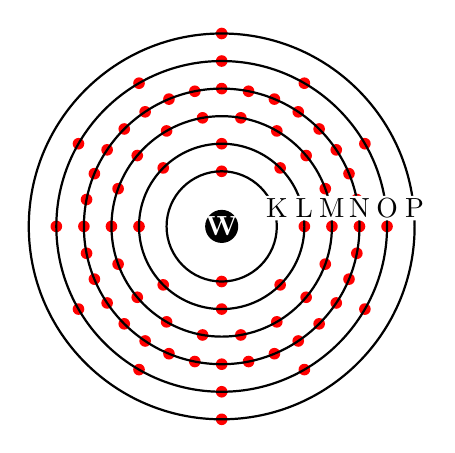
\begin{tikzpicture}[scale=.7]
            % Nucleus
            \fill[black] (0,0) circle (0.3);
            \node at (0,0) [white] {\textbf{W}};

            % K-shell
            \foreach \angle in {90,270} {
                \fill[color=red] (0,0) ++(\angle:1) circle (3pt);
            }
            % L-shell
            \foreach \angle in {0,45,...,315} {
                \fill[color=red] (0,0) ++(\angle:1.5) circle (3pt);
            }
            % M-shell
            \foreach \angle in {0,20,...,340} {
                \fill[color=red] (0,0) ++(\angle:2) circle (3pt);
            }
            % N-shell
            \foreach \angle in {0,11.25,...,348.75} {
                \fill[color=red] (0,0) ++(\angle:2.5) circle (3pt);
            }
            % O-shell
            \foreach \angle in {0,30,...,330} {
                \fill[color=red] (0,0) ++(\angle:3) circle (3pt);
            }
            % P-shell
            \foreach \angle in {90,270} {
                \fill[color=red] (0,0) ++(\angle:3.5) circle (3pt);
            }

            % Shell circles + labels
            \foreach \radius/\label in {1/K, 1.5/L, 2/M, 2.5/N, 3/O, 3.5/P} {
                \draw[thick] (0,0) circle (\radius);
                \node[above, fill=white, inner sep=1pt, rounded corners=1pt] at (\radius, 0.1) {\label};
            }
        \end{tikzpicture}
        \end{adjustbox}
        \caption{Bohr model of tungsten (W, Z=74) with electron shells.}
        \label{fig:tungsten_atomic_model_bohr}
    \end{subfigure}%
    \hfill
    % --- (b) Table on the RIGHT ---
    \begin{subfigure}[c]{0.45\linewidth}   % <- align bottom
        \centering
        \begin{adjustbox}{max width=\linewidth}
        \begin{tabular}{cc}
            \toprule
            \textbf{Shell / Subshell} & \textbf{Binding Energy (keV)} \\
            \midrule
            K     & 69.5 \\
            L$_1$ & 12.1 \\
            L$_2$ & 11.5 \\
            L$_3$ & 10.2 \\
            M$_1$ & 2.82 \\
            M$_2$ & 2.30 \\
            M$_3$ & 2.15 \\
            N$_1$ & 0.43 \\
            N$_2$ & 0.32 \\
            N$_3$ & 0.22 \\
            \bottomrule
        \end{tabular}
        \end{adjustbox}
        \caption{Approximate binding energies of tungsten shells/subshells.}
        \label{tab:tungsten_binding_energies}
    \end{subfigure}

    \caption{(a) Tungsten atom schematic and (b) corresponding binding energies.}
    \label{fig:tungsten_combined}
\end{figure}


Although it is not necessary to understand every technical detail of the X-ray
apparatus for the purposes of simulation, this background information allows one
to assess how key simulation parameters influence the resulting X-ray spectrum
and photon behavior.

Figure~\ref{fig:spectrum100kvp} below shows a resulting energy spectrum for an
X-ray tube with a tungsten cathode operated at 100 kVp. It illustrates the
resulting distribution of photon energies, which is shaped by both the material
and the applied voltage. The intensity of the different photon energies is
measured as \emph{spectral fluence} in
\si{\per\square\centi\meter\per\kilo\electronvolt}, which describes the number
of X-ray photons per unit area per unit energy interval. It clearly shows the
two components of the X-ray spectrum: the continuous bremsstrahlung spectrum and
the characteristic radiation peaks:

\begin{figure}[H]
    \centering

    % (a) Without filter
    \begin{subfigure}[t]{0.48\linewidth}
        \centering
        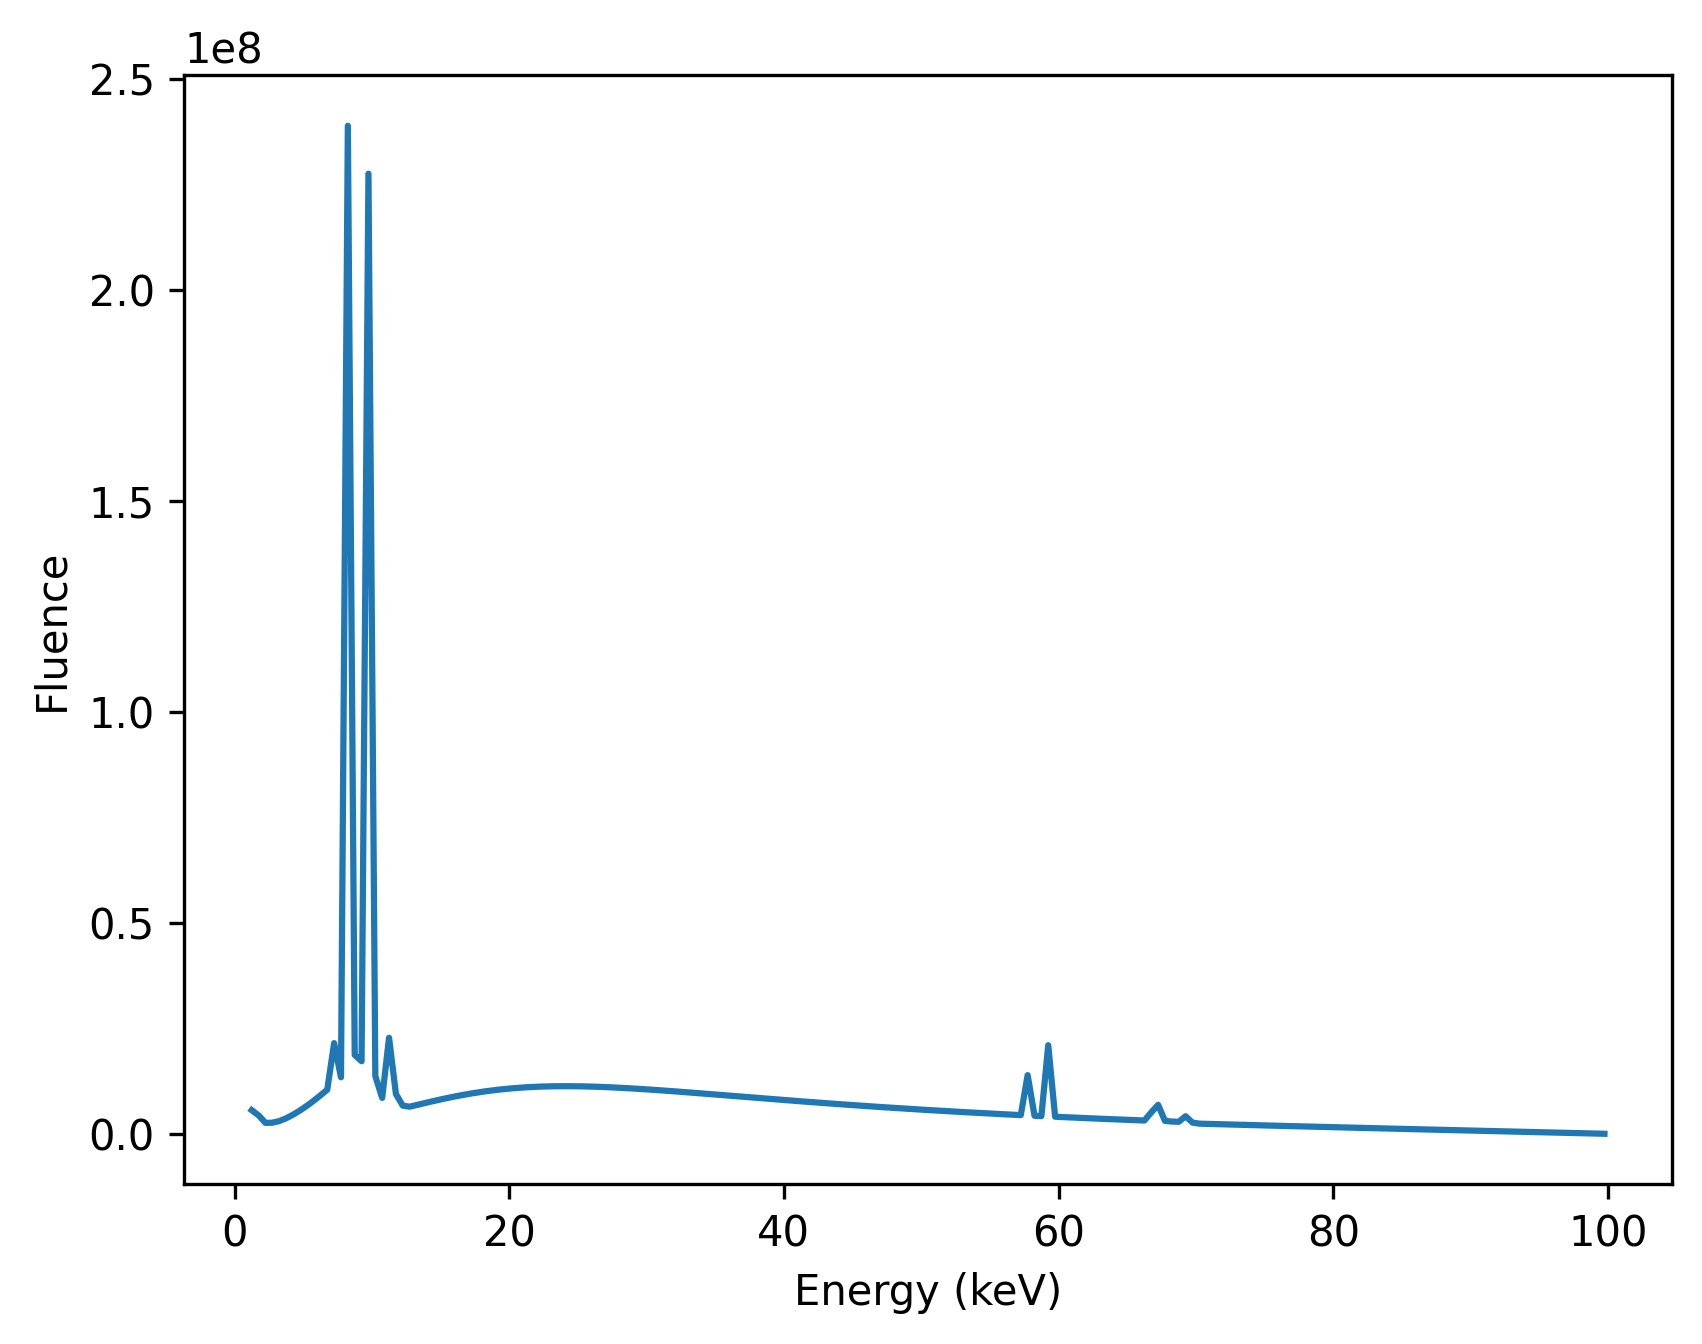
\includegraphics[width=\linewidth]{Figures/spectrum_without_filter.png}
        \caption{Without additional filter.\\
        \emph{Features:} continuous bremsstrahlung up to 100\,kVp; pronounced L-lines ($\sim$8-12\,keV) and K-lines ($\sim$59-67\,keV).}
        \label{fig:spectrum100kvp}
    \end{subfigure}\hfill
    % (b) With filter
    \begin{subfigure}[t]{0.48\linewidth}
        \centering
        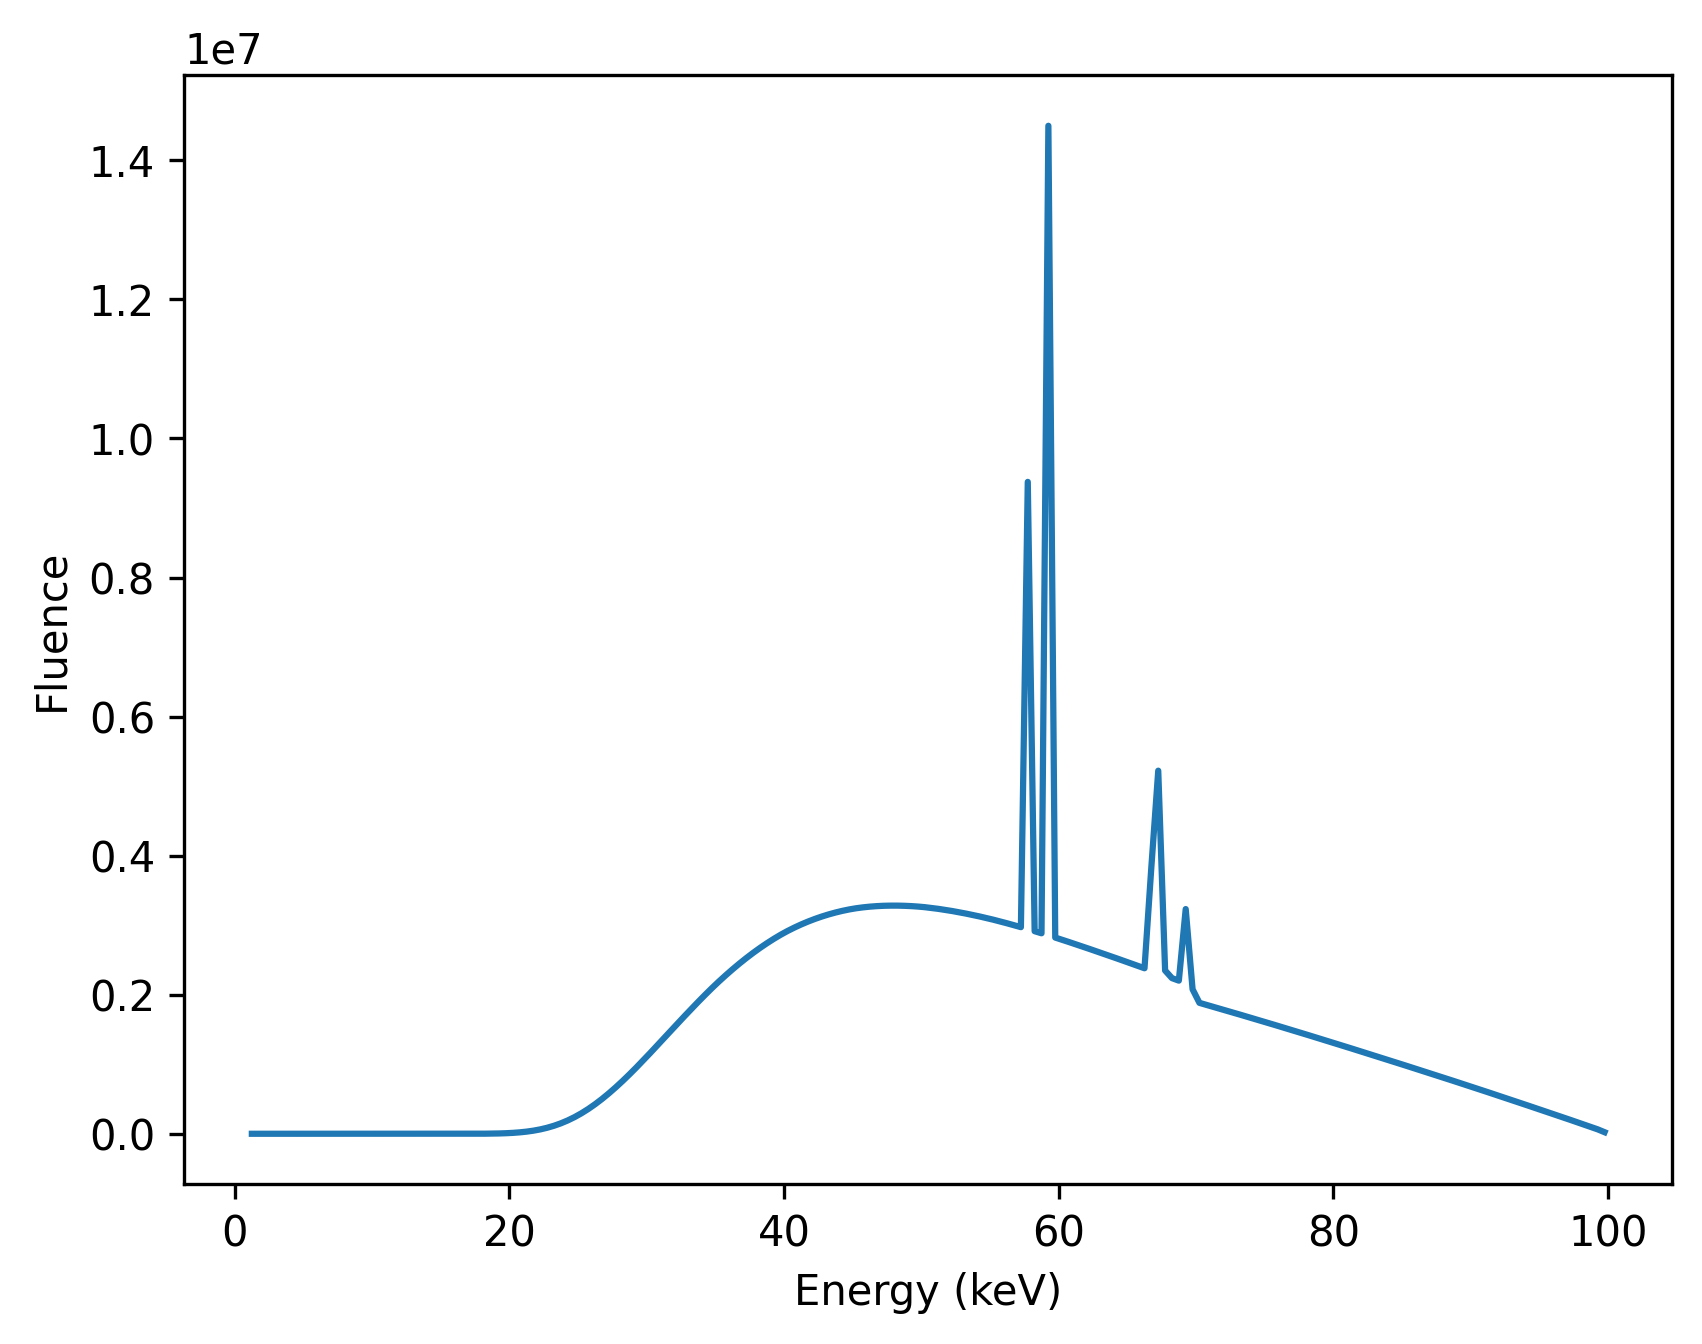
\includegraphics[width=\linewidth]{Figures/spectrum_with_filter.png}
        \caption{With filter (1\,mm Al + 0.2\,mm Cu).\\
        \emph{Effect:} removal of low-energy photons (beam hardening); suppressed L-lines; continuum shifted toward higher mean energy.}
        \label{fig:spectrum100kvp_with_filter}
    \end{subfigure}

    \caption{X-ray spectra for a tungsten anode at 100\,kVp: (a) without and (b) with added filtration. The filter selectively attenuates low-energy photons, reducing patient dose while preserving higher-energy components. Both spectra were generated using \emph{SpekPy} \cite{spekpy}.}
    \label{fig:spectrum100kvp_comparison}
\end{figure}

The applied filter in Figure~\ref{fig:spectrum100kvp_with_filter} effectively
removes low-energy photons below approximately 30\,keV, which would otherwise
contribute to patient dose without enhancing image quality, as low energy
photons are likely to be absorbed superficially. The filter thus "hardens" the
beam by increasing its mean energy, which improves penetration and reduces
scatter. The characteristic K-lines remain prominent, even though their
intensity is slightly reduced due to the filter's attenuation.

%-------------------------------------------------------------------------------
%	SECTION 3
\section{Photon Generation}
%-------------------------------------------------------------------------------

In the context of Monte Carlo simulations, photons are generated with initial
positions, directions and energies that reflect the physical properties of the
X-ray source and the imaging setup.

\subsection{Initial Photon Energy}
\label{sec:photon_energy}
The initial photon energy is sampled according to the X-ray tube spectrum as
described in Section~\ref{sec:xray_tube_spectrum}. As in
Figure~\ref{fig:spectrum100kvp_comparison}, the spectrum maps the photon energy
to the according frequency. In the simulation applied in this thesis, the
spectra are generated utilizing \emph{SpekPy}
\cite{spekpy,poludniowski2021spekpy}.

The actual energies of the emitted photons in the simulation are then determined
by \emph{inverse transform sampling} \cite[Chapter~4]{muller2012monte}. To
determine a matching random variable with the desired distribution, the
following steps need to be made:

\begin{enumerate}[label=(\roman*)]
    \item Construct the appropriate probability density function from the given
    spectrum.
    \item Compute the \ac{cdf} $F$ from the probability density function.
    \item Determine the generalized inverse of the \ac{cdf} $F^{-1}$ as defined
    below.
    \item Sample a uniformly distributed random variable $U$ on the interval
    $[0,1]$ and compute the photon energy as $E = F^{-1}(U)$.
\end{enumerate}

To get the probability density function from the given spectrum, the fluences
$w_i$ of the energies $e_i$ in the spectrum are normalized such that
\begin{equation*}
    p_i = \frac{w_i}{\sum_j w_j}\,.
\end{equation*}
Now, the \ac{cdf} $F:\mathbb{R}\to[0,1]$ can be computed as
\begin{equation*}
    F(e_i) = \mathbb{P}[E \leq e_i] = \sum_{j \leq i} p_j\,.
\end{equation*}
It is clear that $F(e_i)$ is monotonically increasing with $F(-\infty) = 0$ and
$F(\infty) = 1$. The generalized inverse is defined as follows:

\begin{definition}[Generalized Inverse] \ \\
    Let $f: \mathbb{R} \to \mathbb{R}$ be a monotonically increasing function. The \emph{generalized inverse} $f^{-1}: \mathbb{R} \to \mathbb{R}$ is defined as
    \begin{equation*}
        f^{-1}(y) = \inf\{x \in \mathbb{R} : f(x) \geq y\}\,.
    \end{equation*}
\end{definition}

\begin{remark}
    For discrete distributions with support $\{x_1, \ldots, x_M\}$ with $x_1<\ldots<x_M$, the generalized inverse can be explicitly expressed as:
    \begin{equation*}
        f^{-1}(y) = \begin{cases}
            -\infty, & y =0 \\
            x_i, & f(x_{i-1}) < y \leq f(x_i) \\
            x_M, & y=1
        \end{cases}
    \end{equation*}
\end{remark}

As $F$ is monotonically increasing, the generalized inverse $F^{-1}$ exists and
is also monotonically increasing. The photon energies are then sampled via
\begin{equation*}
    E = F^{-1}(U)\,,
\end{equation*}
where $U$ is a uniformly distributed random variable on the interval $[0,1]$.

The following theorem shows that the evaluation of the inverse \ac{cdf} of the
uniformly distributed random variable $U \sim \mathcal{U}(0,1)$ inherits the
desired distribution of the spectrum.

\begin{theorem} \ \\
Let $F:\mathbb{R}\to[0,1]$ be a cumulative distribution function and $F^{-1}$
its generalized inverse. Then for a random variable $X$ generated by
\begin{equation*}
    X := F^{-1}(U)
\end{equation*}
for $U \sim \mathcal{U}(0,1)$, it holds that $X$ has cumulative distribution function $F$, i.e.,
\begin{equation*}
    \mathbb{P}[X \leq x] = F(x), \quad \text{for all } x \in \mathbb{R}.
\end{equation*}
\end{theorem}

\begin{proof}\ \\
It needs to be shown that
\begin{equation*}
    \mathbb{P}[F^{-1}(U) \leq x] = F(x)\,.
\end{equation*}
It is clear that $\mathbb{P}[U\leq F(x)] = F(x)$ for all $x \in \mathbb{R}$,
since $U \sim \mathcal{U}(0,1)$.

Now let $u\in(0,1)$ and $x\in\mathbb{R}$ and $F(x)\geq u$. Then $F^{-1}(u) \leq
x$ as $x\in\{z\in\mathbb{R}:F(z)\geq u\}$. Now let
$x>F^{-1}(u)=\inf\{z\in\mathbb{R}:F(z)\geq u\}$. Since $F$ is non-decreasing, it
holds that $F(x)\geq u$. Lastly, let $x=F^{-1}(u)$. Since $F$ is additionally
right-continuous, it holds that $F(x)\geq u$. Thus, it was shown that 
\begin{equation*}
    \mathbb{P}[F^{-1}(U)\leq x] = \mathbb{P}[X\leq x] = \mathbb{P}[U\leq F(x)] = F(x)\,.
\end{equation*}
\end{proof}

This proof is adapted from \cite{aneuki}

\begin{remark} \ \\
    In the continuous setting with a distribution with strictly positive
    probability density function and thus, strictly increasing \ac{cdf}, the
    generalized inverse coincides with the usual inverse.
\end{remark}


\subsection{Photon Position and Direction}
\label{sec:photon_position_direction}

In addition to the photon energy at emission, its initial position and direction
must be set. Within the simulation framework, two different source models are
considered:

\begin{enumerate}
    \item \textbf{Point Source:} Photons are emitted from a single point in
    space, typically representing the focal spot of the X-ray tube. The emission
    direction is sampled uniformly within a conical emission region defined by
    the half-opening angle $\Theta\in [0^\circ,90^\circ]$.
    \item \textbf{Extended Source:} Photons are emitted from a finite
    rectangular area on a plane, with each photon initially traveling
    perpendicular to this plane.
\end{enumerate}

\paragraph{Point Source} \ \\
This model reflects the global imaging geometry of an X-ray tube with a
point-like focal spot and divergent beam. In line with common practice (e.g.\
Geant4's angular settings~\cite{geant4}), photon directions are sampled
uniformly on a spherical cap, i.e.\ uniformly in the solid angle.

All photons are emitted from a fixed source position
$\mathcal{S}=(\mathcal{S}_1,\mathcal{S}_2,\mathcal{S}_3)\in\mathbb{R}^3$. To
describe the corresponding probability measure, recall that the unit sphere
$S^2$ in spherical coordinates is parameterized by
\[
x=\sin\theta\cos\phi,\quad y=\sin\theta\sin\phi,\quad z=\cos\theta,
\]
with $\theta\in[0,\pi]$ and $\phi\in[0,2\pi)$. The induced surface element on
$S^2$ is given by
\[
d\Omega = \sin\theta\,d\theta\,d\phi .
\]
% see for instance \cite[Theorem~5-6]{spivak2018calculus}. 
A uniform distribution
on the spherical surface thus corresponds to a constant density with respect to
this measure. 


% Restricting the support to the spherical cap
% $\{\theta \in [0,\Theta]\}$ gives the normalized density
% \[
% f(\theta,\phi) = \frac{1}{2\pi\,(1-\cos\Theta)} \quad \text{for } 
% \theta\in[0,\Theta],\ \phi\in[0,2\pi).
% \]

For sampling, one draws $u_1,u_2\sim\mathcal{U}(0,1)$ and sets
\begin{equation*}
    \phi = 2\pi u_2,\qquad
    \cos\theta = 1 - u_1\,(1-\cos\Theta),\qquad
    \theta = \arccos \bigl(1-u_1(1-\cos\Theta)\bigr),
\end{equation*}
leading to the direction vector
\begin{equation*}
    \vec{d}=\bigl(\sin\theta\cos\phi,\; \sin\theta\sin\phi,\; \cos\theta\bigr).
\end{equation*}

This procedure yields a conical beam with half-opening angle $\Theta$ whose
directions are uniformly distributed over the spherical cap surface. Photon
energies are sampled independently from the spectrum as described above.
Figure~\ref{fig:cone_sampling} illustrates the resulting geometry.

\begin{figure}[H]
\centering
\begin{tikzpicture}[scale=.8, >=Latex, line cap=round, line join=round, every node/.style={font=\small}]
\pgfmathsetmacro{\R}{2.8}
\pgfmathsetmacro{\ang}{40}

\pgfmathsetmacro{\ycap}{\R*cos(\ang)}
\pgfmathsetmacro{\acap}{\R*sin(\ang)}
\pgfmathsetmacro{\hcap}{\R-\ycap}

\coordinate (O)  at (0,0);
\coordinate (N)  at (0,\R);
\coordinate (RO) at (\ycap,\acap);
\coordinate (RU) at (\ycap,-\acap);

% \draw[thick] (O) circle (\R);

\shade[ball color=white!99.9!gray, opacity=0.3] (O) circle (\R); % very light
\fill[blue!40, opacity=0.35]
    (RO) arc[start angle=90, end angle=-90, x radius=.05*\R, y radius=\acap]
    arc[start angle=-\ang, end angle=\ang, radius=\R] -- cycle;
\fill[blue!40, opacity=0.35]
    (\ycap,0) ellipse [x radius=0.18, y radius=\acap];

\draw[dashed, blue] (O) -- (RO);
\draw[dashed, blue] (O) -- (RU);
\draw[dashed, black] (O) -- (\R,0);

\pgfmathsetmacro{\ppp}{cos(\ang)}
\pgfmathsetmacro{\qqq}{sin(\ang)}
\draw[thin] (1,0) arc[start angle=0, end angle=\ang, radius=1] -- (\ppp,\qqq);
\draw[thin] (1,0) arc[start angle=0, end angle=-\ang, radius=1] -- (\ppp,-\qqq);


\pgfmathsetmacro{\rrr}{\R*cos(\ang)}
\pgfmathsetmacro{\sss}{\R*sin(\ang)}
\draw[thin, color=green!60!black] (\R,0) arc[start angle=0, end angle=-20, radius=\R] -- (O);
\fill[green!60!black, opacity=0.2] (\R,0) arc[start angle=0, end angle=-20, radius=\R] -- (O) -- cycle;
\node[left=1pt] at ($ (\R,0)!0.2!(\rrr,-\sss) $) {$\theta$};
\pgfmathsetmacro{\ttt}{\R*cos(20)}
\pgfmathsetmacro{\uuu}{\R*sin(20)}
\draw[thin, color=green!60!black] (0,0) -- (\ttt,-\uuu);
\fill[green!60!black] (\ttt,-\uuu) circle (2pt);

\pgfmathsetmacro{\vvv}{\acap}
\draw (RO) arc[start angle=90, end angle=270, x radius=.18, y radius=\vvv];
\draw[dashed] (RO) 
    arc[start angle=90, end angle=270, x radius=-.18, y radius=\vvv];

\fill (O) circle (2pt);
\node[left=0.5pt] at ($ (1,0)!0.4!(\ppp,-\qqq) $) {$\Theta$};
\node[left=0.5pt] at ($ (1,0)!0.4!(\ppp,\qqq) $) {$\Theta$};
\end{tikzpicture}
\caption{Sampling of photon directions uniformly within a cone defined by the half-opening angle $\Theta$.}
\label{fig:cone_sampling}
\end{figure}

In Geant4's \texttt{General Particle Source}, this corresponds to
\emph{isotropic} angular sampling restricted to a cone via min/max $\theta$ and
$\phi$ (e.g.\ \texttt{/gps/ang/type iso}, \texttt{/gps/ang/mintheta 0},
\texttt{/gps/ang/maxtheta $\Theta$}, \texttt{/gps/ang/minphi 0},
\texttt{/gps/ang/maxphi 360 deg}).


\paragraph{Extended Source} \ \\
In contrast, the finite planar source serves primarily as an analytical model.
It describes a local view of the photon--phantom interaction and is employed to
study the influence of source extension on scattering and attenuation effects.

The initial position of a photon is sampled uniformly on the rectangular surface
of the source. For a rectangular source with vertices $P_1,P_2,P_3,P_4 \in
\mathbb{R}^3$ with $\overrightarrow{P_1 P_2} \parallel \overrightarrow{P_3 P_4}$
and $\overrightarrow{P_1 P_4} \parallel \overrightarrow{P_2 P_3}$ being
parallel, the initial position of a photon is determined by two random variables
$u_1,u_2 \sim \mathcal{U}(0,1)$:
\begin{equation*}
    A_0 = P_1 + u_1 \cdot (P_2-P_1) + u_2 \cdot (P_4-P_1) \, .
\end{equation*}
This yields a uniform distribution of starting points over the rectangular
surface. The emission direction of each photon is then set to the unit normal
vector of the source plane, which is aligned with the detector plane, thus
representing a parallel beam geometry.

Such a rectangular planar source model is also supported in Geant4's
\texttt{General Particle Source}, where planar shapes (square or rectangle) can
be chosen for the position distribution and combined with a \emph{planar}
angular type to enforce emission perpendicular to the plane (see
\texttt{/gps/pos/type Plane}, \texttt{/gps/pos/shape Rectangle},
\texttt{/gps/ang/type planar}). This configuration is commonly employed in
benchmark simulations to model collimated or extended X-ray beams.

\qquad

Within this thesis, the experiments were conducted to simulate an X-ray tube
with the parameters listed in Table~\ref{tab:xray_params}.

\begin{table}[H]
    \centering
    \begin{tabular}{ll}
        \toprule
        \textbf{Parameter}      & \textbf{Value} \\
        \midrule
        Tube voltage            & 30--120\,kVp \\
        Anode material          & Tungsten \\
        Filtration              & 1\,\si{\milli\meter} Aluminum (Al),
        0.2\,\si{\milli\meter} Copper (Cu) \\
        Target angle            & 10--60\textdegree \\
        \bottomrule
    \end{tabular}
    \caption{Parameters used to generate the X-ray spectrum with \emph{SpekPy}.}
    \label{tab:xray_params}
\end{table}


% ------------------------------------------------------------------------------
\section{Scattering and Attenuation}
\label{sec:scattering_attenuation}
%-------------------------------------------------------------------------------

Following their emission from the X-ray source, photons traverse space until
they encounter matter, where various interaction processes may occur. The
subsequent section outlines the fundamental mechanisms of photon interactions
with matter. The interaction relevant for medical imaging results in a reduction
of radiation intensity, which corresponds to a decreased number of photons
reaching the detector. Here, X-ray photons may be fully absorbed by
\emph{photoelectric absorption} or undergo either \emph{elastic scattering}
(Rayleigh) or \emph{inelastic scattering} (Compton) as they interact with
matter. In the subsequent sections, these effects will be explained. These
processes depend on the photon energy and the atomic molecules in the material
respecting the density and molecular distribution of the material. A
visualization of these interaction mechanisms is shown in
Figure~\ref{fig:tungsten_atomic_model}.

\begin{figure}[H]
    \centering
    \begin{minipage}[t]{0.3\textwidth}
        \raggedright
        \begin{tikzpicture}[scale=.8]
            \draw[decorate, decoration=snake, {Latex[scale=1.5]}-, shorten <=-10] (2.5,2.3) -- (-2.5,2.3) node[left, xshift=-4pt] {\small$\gamma$};
            \fill[black] (0,0) circle (0.3);
            \foreach \angle in {90, 270} {
                \fill[color=blue] (0,0) ++(\angle:1) circle (3pt);
            }
            \foreach \angle in {0, 45, 90, 135, 180, 225, 270, 315} {
                \fill[color=blue] (0,0) ++(\angle:1.5) circle (3pt);
            }
            \foreach \angle in {0, 40, 80, 120, 160, 200, 240, 280, 320} {
                \fill[color=blue] (0,0) ++(\angle:2cm) circle (3pt);
            }
            \foreach \radius in {1,1.5,2}
            {
                \draw[thick] (0,0) circle (\radius);
            }
            \node[below, font=\large] at (0,-2.5) {No Interaction};
        \end{tikzpicture}
    \end{minipage}
    \hspace{2em} % extra horizontal spacing
    \begin{minipage}[t]{0.3\textwidth}
        \raggedleft
        \begin{tikzpicture}[scale=.8]
            \draw[decorate, decoration=snake, segment length=2mm, {Latex[scale=1.5]}-, shorten <=-10] (2.5,-.15) -- (.25,-.7) -- (-2.5,-.25) node[left, xshift=-4pt] {\small$\gamma$};
            \fill[black] (0,0) circle (0.3);
            \foreach \angle in {90, 270} {
                \fill[color=blue] (0,0) ++(\angle:1) circle (3pt);
            }
            \foreach \angle in {0, 45, 90, 135, 180, 225, 270, 315} {
                \fill[color=blue] (0,0) ++(\angle:1.5) circle (3pt);
            }
            \foreach \angle in {0, 40, 80, 120, 160, 200, 240, 280, 320} {
                \fill[color=blue] (0,0) ++(\angle:2cm) circle (3pt);
            }
            \foreach \radius in {1,1.5,2}
            {
                \draw[thick] (0,0) circle (\radius);
            }
            \node[below, font=\large] at (0,-2.5) {Rayleigh Scattering};
        \end{tikzpicture}
    \end{minipage}
    \par\vspace{3em} % more vertical space
    \begin{minipage}[t]{0.3\textwidth}
        \raggedright
        \begin{tikzpicture}[scale=.8]
            \draw[decorate, decoration=snake] (0,1) -- (-2.5,2.1) node[left, xshift=-4pt] {\small$\gamma$};
            \draw[thick, -{Latex[scale=1.5]}, shorten >=5] (0,1) --
            (2.5, .7) node[draw, circle, fill=black, minimum size=5pt, inner
            sep=0pt] {} node[xshift=10pt, yshift=2pt] {\small$e^\text{-}$};
            \foreach \angle in {90, 270} {
                \fill[color=blue] (0,0) ++(\angle:1) circle (3pt);
            }
            \foreach \angle in {0, 45, 90, 135, 180, 225, 270, 315} {
                \fill[color=blue] (0,0) ++(\angle:1.5) circle (3pt);
            }
            \foreach \angle in {0, 40, 80, 120, 160, 200, 240, 280, 320} {
                \fill[color=blue] (0,0) ++(\angle:2cm) circle (3pt);
            }
            \foreach \radius in {1,1.5,2}
            {
                \draw[thick] (0,0) circle (\radius);
            }
            \fill[black] (0,0) circle (0.3);
            \node[below, font=\large] at (0,-2.5) {Photoelectric Absorption};
        \end{tikzpicture}
    \end{minipage}
    \hspace{2em}
    \begin{minipage}[t]{0.3\textwidth}
        \raggedleft
        \begin{tikzpicture}[scale=.8]
            \draw[decorate, decoration=snake, segment length=2mm] (.3,-2) --
            (-2.5,-2) node[left, xshift=-4pt] {\small$\gamma$};
            \draw[decorate, decoration=snake, segment length=4mm, -{Latex[scale=1.5]}, shorten >=-6] (.3,-2) -- (2.0,-1.5);
            \draw[thick, -{Latex[scale=1.5]}, shorten >=5] (.3,-2) -- (2.5,-2.5)
            node[draw, circle, fill=black, minimum size=5pt, inner sep=0pt] {}
            node[xshift=10pt, yshift=2pt] {\small$e^\text{-}$};
            \fill[black] (0,0) circle (0.3);
            \foreach \angle in {90, 270} {
                \fill[color=blue] (0,0) ++(\angle:1) circle (3pt);
            }
            \foreach \angle in {0, 45, 90, 135, 180, 225, 270, 315} {
                \fill[color=blue] (0,0) ++(\angle:1.5) circle (3pt);
            }
            \foreach \angle in {0, 40, 80, 120, 160, 200, 240, 280, 320} {
                \fill[color=blue] (0,0) ++(\angle:2cm) circle (3pt);
            }
            \foreach \radius in {1,1.5,2}
            {
                \draw[thick] (0,0) circle (\radius);
            }
            \node[below, font=\large] at (0,-2.5) {Compton Scattering};
        \end{tikzpicture}
    \end{minipage}
    \caption{Principles from photon interaction with matter similar to \cite[Chapter 7]{medicalImagingSystemsIntro2019:}}
    \label{fig:tungsten_atomic_model}
\end{figure}

The attenuation of X-ray photons arises from physical processes that alter their
number, direction or energy as they interact with matter. These interactions
occur at the level of individual photons and are highly dependent on the photon
energy. This section presents an overview of the primary interaction mechanisms
relevant to attenuation as in \cite{medicalImagingSystemsIntro2019:}.

For correctness, in the simulations it is further assumed that the X-ray
photons are propagating through air before entering and after exiting the
phantom, where the possible interactions with molecules in the air are neglected.

\subsection{Free Path Length}

All mentioned interaction processes - the photoelectric effect, Compton
scattering and Rayleigh scattering - are probabilistic in nature. Their
attenuation is stochastically characterized by the \emph{mass attenuation
coefficient} $\tilde{\mu}$ in \si{\square\centi\metre\per\gram}. The attenuation
coefficient reflects the composition of the material and the energy of the
photon.  Even though, the attenuation is depending on the density of the
material, the \emph{mass attenuation coefficients} do not depend on the density.

Therefore, the \emph{linear attenuation coefficient} $\mu$ in
\si{\per\centi\metre}, which is then applied within the Beer--Lambert law, is
obtained by multiplying the mass attenuation coefficient $\tilde{\mu}$ with the
density $\rho$ of the material:

$$\mu(x,E) = \rho(x) \cdot \tilde{\mu}(x,E)$$

For comprehensibility, the dependence on the material and density is implicitly
expressed by the Cartesian coordinates $x$ of the photon position. This is
justified, as the material and density also depend on the spatial location
within the phantom. Therefore, a simple and not further mentioned helper
function is returning the \emph{linear attenuation coefficient} $\mu$ for a
given position $x$ and energy $E$. The coefficients are summarized in
Table~\ref{tab:attenuation_coefficients}.

\begin{table}[H]
    \centering
    \begin{tabular}{lcc}
        \toprule
        \textbf{Interaction Type} & \textbf{Attenuation Coefficient} \\
        \midrule
        Photoelectric Effect & $\mu_{\text{PE}}(x,E)$ \\
        Rayleigh Scattering & $\mu_{\text{RS}}(x,E)$ \\
        Compton Scattering & $\mu_{\text{CS}}(x,E)$ \\
        \bottomrule
    \end{tabular}
    \caption{Attenuation coefficients for different photon interaction mechanisms.}
    \label{tab:attenuation_coefficients}
\end{table}

The linear attenuation coefficient $\mu(x,E)$ is the sum of the individual
linear attenuation coefficients for interactions:

$$\mu(x,E) = \mu_{\text{PE}}(x,E) + \mu_{\text{RS}}(x,E) +
\mu_{\text{CS}}(x,E)$$

For the simulations within this thesis, the attenuation coefficients for the
respective phantoms are retrieved from the \emph{XCOM Photon Cross Sections
Database} \cite{nistXCOM}. XCOM is standard database provided by the National
Institute of Standards and Technology (NIST) that comprehends attenuation
coefficients for elements, compounds, and mixtures at energies ranging from
1\,keV to 100\,GeV.

For the behavior of X-ray photons two main effects are considered:
\begin{itemize}
    \item \textbf{Attenuation:} The photon may be absorbed or scattered.
    \item \textbf{No Interaction:} The photon may pass through the phantom
    without any interaction.
\end{itemize}

An interaction may occur at some point along the ray. The probability that a
phantom survives from a certain point $A$ to another point $B$ without any
interaction, is described as follows \cite{bezug2014computed}:

$$\mathcal{P}(A, \overrightarrow{AB},E) = \exp\bigg[-\int_{A}^{B}{A +
\mu\bigg(\frac{s}{\|\overrightarrow{AB}\|}(B-A),E \bigg)\,ds}\bigg]$$

The free path length of a photon is the distance it travels before interacting
with matter. To sample the free path length of a photon, one can project the
photon within a given direction $\vec{\omega}$ from its current position $A$ to
the detector position $\hat{C}$, as shown in Figure~\ref{fig:exit_point}. Then
a random variable $U \sim \mathcal{U}(0,1)$ is sampled.

\begin{itemize}
    \item If $U < \mathcal{P}(A, \vec{\omega}, E)$, the photon reaches the detector without any interaction.
    \item If $U \geq \mathcal{P}(A, \vec{\omega}, E)$, the photon interacts with matter after traveling the free path length $t$. The free path length $t$ is then determined by solving the equation 
    $$\int_{0}^{t}{\mu(A+s\cdot\vec{\omega},E)\,ds} = -\log(1-U)$$
\end{itemize}

\begin{figure}[H]
    \centering
    \begin{tikzpicture}[scale=1]
        \draw[color=gray, fill=gray!30] plot[smooth cycle] coordinates {(-2,0) (-2.5,1.5) (0,3) (3,1.5) (4,-1) (3,-2) (-2,-2.5)};
        \filldraw[fill=black] (-5,.5) circle (4pt) node[above, inner sep=7pt] {$S$};
        \node[below, inner sep=7pt] at (-3.5,.25) {$\vec{v}$};
        \draw[thick] (-5,.5) -- (-2,0);
        \filldraw[fill=black] (-2,0) circle (4pt) node[above, inner sep=7pt] {$A_0$};
        \draw[thick] (-2,0) -- (4,-1);
        \filldraw[fill=black] (4,-1) circle (4pt) node[above, inner sep=7pt] {$C$};
        \draw[thick, -{Latex[scale=1.5]}] (4,-1) -- (7,-1.5);
        \filldraw[fill=black] (7,-1.5) circle (4pt) node[left, below, inner sep=7pt] {$\hat{C}$};  
        \filldraw[
            draw=teal,
            pattern={Lines[angle=0, distance=4pt, line width=0.5pt]},
            pattern color=teal
        ] (7,-4) rectangle (7.3,4);
        \node[rotate=90, anchor=south, color=teal] at (8,0) {Detector Grid};

        % \node[above] at (-.5,.5) {$A_0$};
    \end{tikzpicture}
    \caption{Illustration of the entry and exit point of the ray of a photon without interaction.}
    \label{fig:exit_point}
\end{figure}


\subsection{Compton Scattering}
\label{sec:physicsComptonScattering}
\emph{Compton scattering} is the most dominant interaction mechanism for X-ray
photons in tissue \cite[Chapter 7]{medicalImagingSystemsIntro2019:}. It occurs
when a X-ray photon with considerably higher energy than the binding energy of
an outer shell electron collides with this electron. This interaction results in
a transfer of energy and momentum. The electron is ejected from the atom, while
the incoming photon is scattered at an angle and its energy is reduced.

A portion of the incident photon energy is transferred to the electron, which is
referred to as the "recoil electron" or Compton electron. The interaction
produces a positive ion, the "recoil electron" and a scattered photon. If the
deflection angle of the scattered photon is small, most of the energy is
retained by the scattered photon. The deflection angle can vary from 0 to 180
degrees, depending on the energy transfer during the interaction. Thus, the
photon can be scattered in any direction, with the probability of scattering at
smaller angles being higher than at larger angles.

For the distribution of the scattering angle $\theta$ of the scattered photons
in the differential cross section, we apply the formula derived by \emph{Klein
and Nishina} in 1928. This equation describes the angular distribution of X-ray
photons in Compton scattering, assuming the electron is initially free and
stationary. The relation between energy loss and photon deflection is determined
from conservation of momentum and energy between the photon and the recoiling
electron \cite{hubbell1969photon,klein1928scattering}.

The Klein--Nishina formula provides the differential cross section for Compton
scattering with scattering angle $\theta$, initial photon energy $E$ and
scattered photon energy $E'$. Thus, $\theta$ is the angle between the direction
of the incident photon and the direction of the scattered photon.

$$ \frac{d\sigma}{d\Omega} = \frac{r_e^2}{2}
\bigg(\frac{E^\prime}{E}\bigg)^2 \bigg(\frac{E}{E^\prime} + \frac{E^\prime}{E} -
\sin^2(\theta)\bigg) $$

Further, the relation
between the energies of the incident photon $E$ and the scattered photon $E'$ is
given by the \emph{Compton formula}:

\begin{equation}
    E' = \frac{E}{1 + \frac{E}{m_e c^2} (1 - \cos \theta)} = \frac{E}{1 + k(1 - \cos \theta)}
    \label{eq:compton_formula}
\end{equation}

where $k=\tfrac{E}{m_ec^2}$ is used for readability.
Here, $m_ec^2$ denotes the electron rest energy, which is approximately $0.511 MeV$ and $r_e$ denotes the classical
electron radius. Together, this yields the following form of the Klein-Nishina formula:

\begin{equation}
    \label{eq:kleinNishina}
    \frac{d\sigma}{d\Omega} (\theta, k)= \frac{1}{2} r_e^2 
    \frac{1}{(1 + k(1 - \cos \theta))^2} \left( 1 + \cos^2 \theta + 
    \frac{k^2 (1 - \cos \theta)^2}{1+ k(1 - \cos \theta)} \right),
\end{equation}

The Klein--Nishina formula describes the angular distribution of the scattering
probability. Here, $\sigma$ denotes the scattering cross section, which
quantifies the probability of an interaction by the effective area for
scattering, and $\Omega$ denotes the solid angle, describing the
three-dimensional angular space into which the photon may be scattered. The
expression $\tfrac{d\sigma}{d\Omega}$ is thus the \emph{differential cross
section}, which represents the probability density of photons being scattered
into a particular direction. 

For sampling from the Klein-Nishina distribution, we cannot apply the Inverse
Transform Sampling method as described in Section~\ref{sec:photon_energy}, 
since the structure of the Klein-Nishina formula and the dependency of $\theta$
is more complex and does not allow for an analytical inversion.
Instead the method of \emph{acceptance--rejection sampling} is used. 

Acceptance--rejection sampling is a method for generating random samples from a
probability distribution $f(x)$ when direct sampling is difficult. The idea is
to employ a simpler envelope distribution $h(x)$, from which samples can be
drawn efficiently, and which dominates $f(x)$ up to a constant factor. More
precisely, one requires a constant $0< c \leq 1$ such that $c\,f(x) \leq h(x)$
for all $x$. A candidate value $x$ is drawn from $h(x)$, and an auxiliary
uniform random number $u \sim \mathcal{U}(0,1)$ is generated. The sample $x$ is
accepted if $u \leq \tfrac{c\,f(x)}{h(x)}$, otherwise it is rejected and the
procedure is repeated until an acceptance occurs.

The efficiency of the algorithm depends on how tightly $h(x)$ bounds $c\,f(x)$:
the closer the proposal envelope matches the target distribution, the higher the
acceptance rate. Acceptance--rejection sampling is thus most effective when a
proposal distribution can be chosen that both resembles the target distribution
and allows efficient evaluation. For more details, see for instance \cite[Chap 4]{muller2012monte} or \cite[Section 8.1]{leobacher2014introduction}.

To apply the acceptance--rejection sampling method to the Klein-Nishina formula equation~\eqref{eq:kleinNishina}, we first rewrite $\frac{d\sigma}{d\Omega} (\theta, k)$ to $f(k,x)$ using $x=\cos\theta$ and ignore the constant factors which are not relevant for sampling:
\begin{equation}
    f(k,x) = \frac{1}{(1 + k(1 - x))^2} \left( 1 + x^2 + \frac{k^2 (1 - x)^2}{1+ k(1 - x)} \right)
\end{equation}

Following \cite{ozmutlu1992sampling}, we start by choosing an envelope distribution $h(k,x)$ of the form
\begin{equation*}
    h(k,x) = \frac{a(k)}{b(k)-x}
\end{equation*}

with $a(k), b(k)$ to be determined such that the envelope function matches the target function at the boundaries $x=1$ and $x=-1$. This leads to the conditions:

\begin{align*}
    f(k,1) &= 2 = h(k,1) \\
    f(k,-1) &= \zeta(k) = h(k,-1)  \quad \text{ with}\\
     \zeta(k) &= \frac{2(2k^2 + 2k + 1)}{(2k + 1)^3}
\end{align*}

Imposing these endpoint conditions on $h(k,x)=\dfrac{a(k)}{b(k)-x}$, yields
\begin{align*}
\frac{a(k)}{b(k)-1}=2 \quad&\Rightarrow\quad a(k)=2(b(k)-1),\\
\frac{a(k)}{b(k)+1}=\zeta(k) \quad&\Rightarrow\quad \frac{2(b(k)-1)}{b(k)+1}=\zeta(k).
\end{align*}
Solving the second equation for $b(k)$ by multiplying out gives
$$
b(k)=\frac{2+\zeta(k)}{2-\zeta(k)}=\frac{1+\frac{\zeta(k)}{2}}{1-\frac{\zeta(k)}{2}} $$

Thus, the envelope function is given with the values:



\begin{align*}
    h(k,x) &= \frac{a(k)}{b(k)-x} \\
    a(k) &= 2(b(k)-1) \\
    b(k) &= \frac{1+\frac{\zeta(k)}{2}}{1-\frac{\zeta(k)}{2}}
\end{align*}

For the acceptance--rejection method to be applicable, we need to ensure that $c\,f(k,x) \leq h(k,x)$ for all $x \in [-1,1]$ and some constant $0 < c \leq 1$. 

Therefore, consider the ratio $R_k(x)\coloneqq h(k,x)/f(k,x)$ for $x\in[-1,1]$.
Since $f(k,x)>0$ for all $x\in[-1,1]$ (Klein--Nishina is strictly positive) and
$h(k,x)>0$ because $b(k)>1$ which implies $b(k)-x>0$ on $[-1,1]$, we have $R_k(x)>0$
on $[-1,1]$. At the endpoints, $R_k(\pm 1)=1$ by the matching conditions above,
so $c_k\le 1$. Therefore, $h(k,x)\ge c_k\,f(k,x)$ for all $x\in[-1,1]$, with a
uniform constant $c_k \in(0,1]$.

Now the acceptance--rejection method can be applied. To sample the scattering
angle $\theta$, $x=\cos\theta$ is sampled from the distribution $h$ by the
inverse transform method:

The cumulative distribution function of $h$ is
$$
H(x) = \int_{-1}^{x}h(k,t)\,dt=\int_{-1}^x \frac{a}{b-t}\,dt
= a\,\ln\!\left(\frac{b+1}{b-x}\right),
$$
which, after normalization, becomes
$$
\tilde H(x)
= \frac{\ln\!\left(\tfrac{b+1}{\,b-x\,}\right)}
       {\ln\!\left(\tfrac{b+1}{\,b-1\,}\right)}.
$$
Setting $\tilde H(x)=r$ for $r\sim\mathcal U(0,1)$ and solving for $x$ yields
$$
x = b - (b+1)\left(\frac{b-1}{b+1}\right)^{r}.
$$
With the parametrization
$$
b(k) = \frac{1+\frac{\zeta(k)}{2}}{1-\frac{\zeta(k)}{2}}
\quad\Longrightarrow\quad
\frac{b-1}{b+1} = \frac{\zeta(k)}{2},
$$
this simplifies to the final sampling formula
$$
x = b(k) - (b(k)+1)\left(\frac{\zeta(k)}{2}\right)^{r},
$$
for a uniform random variable $r \sim \mathcal{U}(0,1)$. 

This value is accepted if $\frac{f(k,x)}{h(k,x)} \geq u_1$, where $u_1$ denotes a uniform random variable. If the value is not accepted, a new value is sampled until acceptance occurs. The scattering angle $\theta$ is then obtained by $\theta = \arccos(x)$.

Once the scattering angle $\theta$ is sampled, the new energy of the scattered
photon $E'$ can be calculated using the Compton formula:

\begin{equation}
    \label{eq:compton_energy}
    E' = \frac{E}{1 + \frac{E}{m_e c^2} (1 - \cos \theta)}
\end{equation}

Given the scattering angle $\theta$ and an azimuthal angle $\phi=u_2 \cdot 2\pi$
for $u_2\in[0,1]$ denoting a second random value, the new direction
$\vec{\omega}'$ can be obtained by rotating the initial direction $\vec{\omega}$
accordingly. This is achieved by constructing a local orthonormal basis
$\{\vec{e}_1,\vec{e}_2,\vec{\omega}\}$ and expressing the scattered direction as  
\[
    \vec{\omega}' = \cos\theta \, \vec{\omega}
    + \sin\theta \bigl(\cos\phi \, \vec{e}_1 + \sin\phi \, \vec{e}_2\bigr)\,.
\]


\subsection{Rayleigh Scattering}
\emph{Rayleigh scattering} is an elastic scattering process that occurs at low
X-ray energies \cite[Chapter 7]{medicalImagingSystemsIntro2019:}. The incident
photon interacts coherently with bound electrons in the outer shells, driving a
collective oscillation of the electron cloud. The atom then re-radiates a photon
of the same energy (wavelength) but generally in a different direction. Because
the interaction is elastic, no electrons are ejected and no ionization occurs.
At diagnostic energies, the differential cross section is strongly
forward-peaked, so most scattered photons are deflected by small angles.

Although Rayleigh scattering takes place in the X-ray tube, it can be excluded
from the linear attenuation coefficient, as it does not contribute to the
attenuation of the X-ray beam in the same way as Compton scattering or
photoelectric absorption. As described in \cite{poludniowski2022calculating},
the exclusion of Rayleigh scattering from the linear attenuation coefficient is
based on the assumption that the characteristic radiation emitted by the target
is isotropic, meaning it is emitted uniformly in all directions. As the X-ray is
not attenuated by Rayleigh scattering, it is a common assumption to exclude
Rayleigh scattering from the attenuation coefficient.

Therefore, it is justified to neglect Rayleigh scattering in the simulation of
X-ray imaging, as it does not significantly affect the overall attenuation of
the X-ray beam. This simplification allows for a more efficient simulation
without compromising the accuracy of the results.

\bigskip
The physical principles described in this chapter provide the building blocks
for modeling photon transport in X-ray imaging. Based on these laws, the
subsequent Chapter~\ref{chapter10} presents the simulation
framework, combining photon generation, ray traversal, and interaction
mechanisms into a coherent algorithmic structure that integrates \ac{qmc}
sampling strategies.
